\section{Four 4-transpositions}

\begin{theorem}
  There is a single sggi of rank 4 over $A_{11}$ that is composed by 4-transposition. This sggi is represented in the appendix~\ref{rank4-4-4transpositions} (p. \pageref{rank4-4-4transpositions})
\end{theorem}

\begin{proof}
  Here is the common graph with the involutions $\rho_1$.

  \begin{figure}[H]
    \begin{center}
      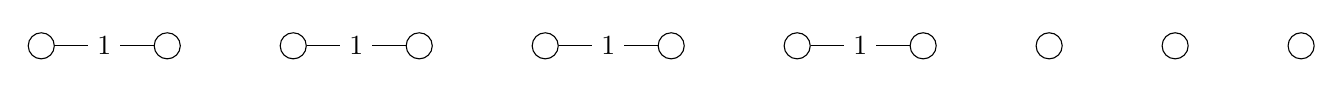
\begin{tikzpicture}[scale=.8]

        \begin{scope}[every node/.style={circle,draw}]
          \node (1)  at (0,0)  {};
          \node (2)  at (2,0)  {};
          \node (3)  at (4,0)  {};
          \node (4)  at (6,0)  {};
          \node (5)  at (8,0)  {};
          \node (6)  at (10,0)  {};
          \node (7)  at (12,0)  {};
          \node (8)  at (14,0)  {};
          \node (9)  at (16,0)  {};
          \node (10) at (18,0)  {};
          \node (11) at (20,0) {};
        \end{scope}

        \begin{scope}[every node/.style={fill=white}]

          \begin{scope}[every edge/.style={draw}]
            \path (1)  edge node {$1$} (2);
            \path (3)  edge node {$1$} (4);
            \path (5)  edge node {$1$} (6);
            \path (7)  edge node {$1$} (8);
          \end{scope}
        \end{scope}

      \end{tikzpicture}
      \caption{}
    \end{center}
  \end{figure}

  \paragraph{}
  The $\rho_3$ edges must be placed. This involution must commute with $\rho_1$. For each pair of $\rho_3$ there are the three usual possibilities: an alternating square, two double edges or one double edge and link two fixed points. Two alternating squares are not possible as is two double edges\footnote{TODO}.

  \paragraph{}
  Thus an alternating square, a double edge and a link between two fixed points must be built.

  \begin{figure}[H]
    \begin{center}
      \begin{tikzpicture}[scale=.8]

        \begin{scope}[every node/.style={circle,draw}]
          \node (1)  at (0,2)  {};
          \node (2)  at (0,0)  {};
          \node (3)  at (2,2)  {};
          \node (4)  at (2,0)  {};
          \node (5)  at (4,0)  {};
          \node (6)  at (6,0)  {};
          \node (7)  at (8,0)  {};
          \node (8)  at (10,0)  {};
          \node (9)  at (14,0) {};
          \node (10) at (12,0) {};
          \node (11) at (16,0) {};
        \end{scope}

        \begin{scope}[every node/.style={fill=white}]

          \begin{scope}[every edge/.style={draw}]
            \path (1)  edge node {$1$} (2);
            \path (3)  edge node {$1$} (4);
            \path (5)  edge[bend left=30] node {$1$} (6);
            \path (7)  edge node {$1$} (8);
            \path (1)  edge node {$3$} (3);
            \path (2)  edge node {$3$} (4);
            \path (5)  edge[bend right=30] node {$3$} (6);
            \path (9)  edge node {$3$} (10);
          \end{scope}
        \end{scope}

      \end{tikzpicture}
      \caption{}
    \end{center}
  \end{figure}


  \paragraph{}
  The involution $\rho_0$ must commute with $\rho_3$. The constraints are more strict than with $\rho_1$ and $\rho_3$. Therefore the same conclusions can be used: $\rho_0$ and $\rho_3$ must form an alternating square double a $\rho_3$ edge and link two points fixed by $\rho_3$. The link must occurs between $\rho_1$ and the fixed point\footnote{TODO}.

  \begin{figure}[H]
    \begin{center}
      \begin{tikzpicture}[scale=.8]

        \begin{scope}[every node/.style={circle,draw}]
          \node (1)  at (0,2)  {};
          \node (2)  at (0,0)  {};
          \node (3)  at (2,2)  {};
          \node (4)  at (2,0)  {};
          \node (5)  at (4,0)  {};
          \node (6)  at (6,0)  {};
          \node (7)  at (8,0)  {};
          \node (8)  at (10,0)  {};
          \node (9)  at (14,0) {};
          \node (10) at (12,0) {};
          \node (11) at (16,0) {};
        \end{scope}

        \begin{scope}[every node/.style={fill=white}]

          \begin{scope}[every edge/.style={draw}]
            \path (9) edge node {$0$} (11);
            \path (1)  edge node {$1$} (2);
            \path (3)  edge node {$1$} (4);
            \path (5)  edge[bend left=30] node {$1$} (6);
            \path (9)  edge node {$1$} (10);
            \path (1)  edge node {$3$} (3);
            \path (2)  edge node {$3$} (4);
            \path (5)  edge[bend right=30] node {$3$} (6);
            \path (7)  edge node {$3$} (8);
          \end{scope}
        \end{scope}

      \end{tikzpicture}
      \caption{}
    \end{center}
  \end{figure}

  \paragraph{}
  But the only unplaced involution will be $\rho_2$. Therefore all connected components need to be able to be connected by a $\rho_2$ component.

  \paragraph{}
  The two squares need to be ajdacent\footnote{TODO}.
  \begin{figure}[H]
    \begin{center}
      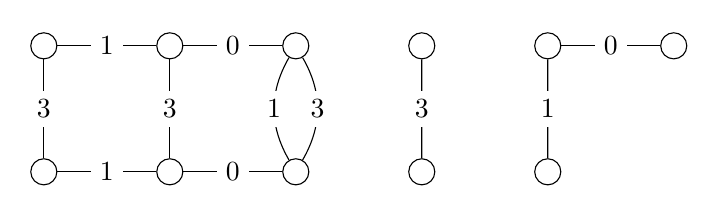
\begin{tikzpicture}[scale=.8]

        \begin{scope}[every node/.style={circle,draw}]
          \node (1)  at (0,2)  {};
          \node (2)  at (2,2)  {};
          \node (3)  at (0,0)  {};
          \node (4)  at (2,0)  {};
          \node (5)  at (4,2)  {};
          \node (6)  at (4,0)  {};
          \node (7)  at (8,2)  {};
          \node (8)  at (8,0)  {};
          \node (9)  at (6,2)  {};
          \node (10) at (6,0)  {};
          \node (11) at (10,2) {};
        \end{scope}

        \begin{scope}[every node/.style={fill=white}]

          \begin{scope}[every edge/.style={draw}]
            \path (2)  edge node {$0$} (5);
            \path (4)  edge node {$0$} (6);
            \path (7)  edge node {$0$} (11);
            \path (1)  edge node {$1$} (2);
            \path (3)  edge node {$1$} (4);
            \path (5)  edge[bend right=30] node {$1$} (6);
            \path (7)  edge node {$1$} (8);
            \path (1)  edge node {$3$} (3);
            \path (2)  edge node {$3$} (4);
            \path (5)  edge[bend left=30] node {$3$} (6);
            \path (9)  edge node {$3$} (10);
          \end{scope}
        \end{scope}

      \end{tikzpicture}
      \caption{}
    \end{center}
  \end{figure}

  \paragraph{}
  The double edge cannot be the single $\rho_3$ because it will be part of an alternating square but that is impossible\footnote{TODO}.

  \begin{figure}[H]
    \begin{center}
      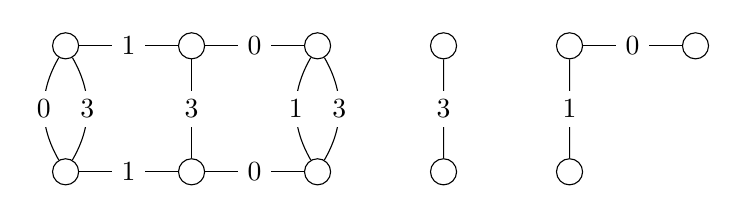
\begin{tikzpicture}[scale=.8]

        \begin{scope}[every node/.style={circle,draw}]
          \node (1)  at (0,2)  {};
          \node (2)  at (2,2)  {};
          \node (3)  at (0,0)  {};
          \node (4)  at (2,0)  {};
          \node (5)  at (4,2)  {};
          \node (6)  at (4,0)  {};
          \node (7)  at (8,2)  {};
          \node (8)  at (8,0)  {};
          \node (9)  at (6,2)  {};
          \node (10) at (6,0)  {};
          \node (11) at (10,2) {};
        \end{scope}

        \begin{scope}[every node/.style={fill=white}]

          \begin{scope}[every edge/.style={draw}]
            \path (2)  edge node {$0$} (5);
            \path (4)  edge node {$0$} (6);
            \path (1)  edge[bend right=30] node {$0$} (3);
            \path (7)  edge node {$0$} (11);
            \path (1)  edge node {$1$} (2);
            \path (3)  edge node {$1$} (4);
            \path (5)  edge[bend right=30] node {$1$} (6);
            \path (7)  edge node {$1$} (8);
            \path (1)  edge[bend left=30] node {$3$} (3);
            \path (2)  edge node {$3$} (4);
            \path (5)  edge[bend left=30] node {$3$} (6);
            \path (9)  edge node {$3$} (10);
          \end{scope}
        \end{scope}

      \end{tikzpicture}
      \caption{}
    \end{center}
  \end{figure}

  \paragraph{}
  It is impossible to link the component on the right to anything with a $\rho_2$ edge without using an alternating square. The involution $\rho_3$ must not be in the new alternating square. There are two places for a square with $\rho_3$ but it is impossible on the right because all $\rho_1$ edges have already been used. And it is impossible on the left because a $\rho_0$ and $\rho_2$ cannot share an edge without an alternating square.

  \paragraph{}
  It is not possible to used $\rho_1$ in the square because a $\rho_0$ and $\rho_2$ edge will be adjacent. The $\rho_0$ must be used.

  \begin{figure}[H]
    \begin{center}
      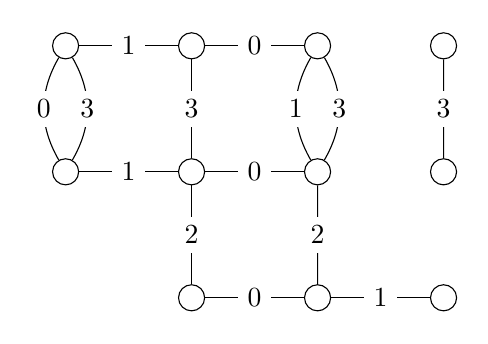
\begin{tikzpicture}[scale=.8]

        \begin{scope}[every node/.style={circle,draw}]
          \node (1)  at (0,2)  {};
          \node (2)  at (2,2)  {};
          \node (3)  at (0,0)  {};
          \node (4)  at (2,0)  {};
          \node (5)  at (4,2)  {};
          \node (6)  at (4,0)  {};
          \node (7)  at (4,-2)  {};
          \node (8)  at (6,-2)  {};
          \node (9)  at (6,2)  {};
          \node (10) at (6,0)  {};
          \node (11) at (2,-2) {};
        \end{scope}

        \begin{scope}[every node/.style={fill=white}]

          \begin{scope}[every edge/.style={draw}]
            \path (2)  edge node {$0$} (5);
            \path (4)  edge node {$0$} (6);
            \path (1)  edge[bend right=30] node {$0$} (3);
            \path (7)  edge node {$0$} (11);
            \path (1)  edge node {$1$} (2);
            \path (3)  edge node {$1$} (4);
            \path (5)  edge[bend right=30] node {$1$} (6);
            \path (7)  edge node {$1$} (8);
            \path (4)  edge node {$2$} (11);
            \path (6)  edge node {$2$} (7);
            \path (1)  edge[bend left=30] node {$3$} (3);
            \path (2)  edge node {$3$} (4);
            \path (5)  edge[bend left=30] node {$3$} (6);
            \path (9)  edge node {$3$} (10);
          \end{scope}
        \end{scope}

      \end{tikzpicture}
      \caption{}
    \end{center}
  \end{figure}

  \paragraph{}
  It still impossible to link the single $\rho_3$ by an alternating square. It must be linked by a single edge. There is single attach point.

  \begin{figure}[H]
    \begin{center}
      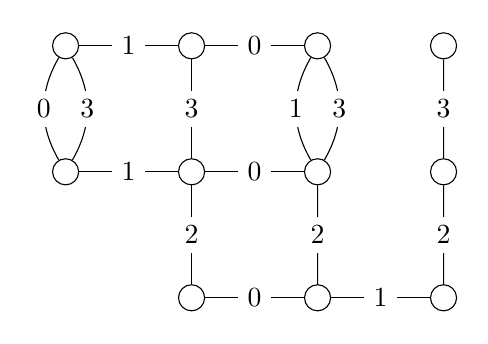
\begin{tikzpicture}[scale=.8]

        \begin{scope}[every node/.style={circle,draw}]
          \node (1)  at (0,2)  {};
          \node (2)  at (2,2)  {};
          \node (3)  at (0,0)  {};
          \node (4)  at (2,0)  {};
          \node (5)  at (4,2)  {};
          \node (6)  at (4,0)  {};
          \node (7)  at (4,-2)  {};
          \node (8)  at (6,-2)  {};
          \node (9)  at (6,2)  {};
          \node (10) at (6,0)  {};
          \node (11) at (2,-2) {};
        \end{scope}

        \begin{scope}[every node/.style={fill=white}]

          \begin{scope}[every edge/.style={draw}]
            \path (2)  edge node {$0$} (5);
            \path (4)  edge node {$0$} (6);
            \path (1)  edge[bend right=30] node {$0$} (3);
            \path (7)  edge node {$0$} (11);
            \path (1)  edge node {$1$} (2);
            \path (3)  edge node {$1$} (4);
            \path (5)  edge[bend right=30] node {$1$} (6);
            \path (7)  edge node {$1$} (8);
            \path (4)  edge node {$2$} (11);
            \path (6)  edge node {$2$} (7);
            \path (8)  edge node {$2$} (10);
            \path (1)  edge[bend left=30] node {$3$} (3);
            \path (2)  edge node {$3$} (4);
            \path (5)  edge[bend left=30] node {$3$} (6);
            \path (9)  edge node {$3$} (10);
          \end{scope}
        \end{scope}

      \end{tikzpicture}
      \caption{}
    \end{center}
  \end{figure}

  \paragraph{}
  The is a single place for the last $\rho_0$ edge.

  \begin{figure}[H]
    \begin{center}
      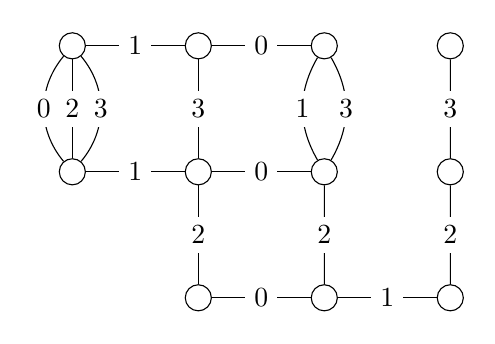
\begin{tikzpicture}[scale=.8]

        \begin{scope}[every node/.style={circle,draw}]
          \node (1)  at (0,2)  {};
          \node (2)  at (2,2)  {};
          \node (3)  at (0,0)  {};
          \node (4)  at (2,0)  {};
          \node (5)  at (4,2)  {};
          \node (6)  at (4,0)  {};
          \node (7)  at (4,-2)  {};
          \node (8)  at (6,-2)  {};
          \node (9)  at (6,2)  {};
          \node (10) at (6,0)  {};
          \node (11) at (2,-2) {};
        \end{scope}

        \begin{scope}[every node/.style={fill=white}]

          \begin{scope}[every edge/.style={draw}]
            \path (2)  edge node {$0$} (5);
            \path (4)  edge node {$0$} (6);
            \path (1)  edge[bend right=40] node {$0$} (3);
            \path (7)  edge node {$0$} (11);
            \path (1)  edge node {$1$} (2);
            \path (3)  edge node {$1$} (4);
            \path (5)  edge[bend right=30] node {$1$} (6);
            \path (7)  edge node {$1$} (8);
            \path (4)  edge node {$2$} (11);
            \path (6)  edge node {$2$} (7);
            \path (8)  edge node {$2$} (10);
            \path (1)  edge node {$2$} (3);
            \path (1)  edge[bend left=40] node {$3$} (3);
            \path (2)  edge node {$3$} (4);
            \path (5)  edge[bend left=30] node {$3$} (6);
            \path (9)  edge node {$3$} (10);
          \end{scope}
        \end{scope}

      \end{tikzpicture}
      \caption{}
    \end{center}
  \end{figure}

  \begin{theorem}
    This sggi is not a C-group
  \end{theorem}

  \begin{proof}
    TODO
  \end{proof}



\end{proof}
